\documentclass{article}
\usepackage[italian]{babel}
\usepackage{graphicx}

% permette agli hypertext di essere cliccabili
\usepackage{hyperref}
\usepackage{longtable}
\usepackage{makecell}

\renewcommand{\arraystretch}{1.6}

\usepackage[raggedrightboxes]{ragged2e}

\usepackage[inline]{enumitem}
\setlist[itemize]{itemsep=0pt, topsep=2pt} % imposta di defualt le opzioni di itemize

\hypersetup{
    colorlinks,
    citecolor=black,
    filecolor=black,
    linkcolor=black,
    urlcolor=black
}
% permette di impostare le dimensioni della pagina
\usepackage[a4paper, total={6in, 9in}]{geometry}

\newcommand{\sskip}{\smallskip \\}
\newcommand{\meskip}{\medskip \\}
\newcommand{\bskip }{\bigskip \\}

\title{Documentazione Object Orientation\\
Sistema di gestione di personale e progetti all'interno di un'azienda }
\author{Roberto Ingenito \and Simone Ingenito \and Lorenzo Sequino}
\date{\today \\ \vspace{2cm} \includegraphics[width=0.5\textwidth]{images/logo.png}}



\usepackage{listings}
\usepackage{xcolor}

\definecolor{codegreen}{rgb}{0,0.6,0}
\definecolor{codegray}{rgb}{0.5,0.5,0.5}
\definecolor{codepurple}{rgb}{0.58,0,0.82}
\definecolor{backcolour}{rgb}{0.95,0.95,0.92}
\lstset{
    language=sql,
    backgroundcolor=\color{backcolour}, 
    keywordstyle=\color{magenta},
    commentstyle=\color{codegreen},
    stringstyle=\color{codepurple},
    basicstyle=\ttfamily\footnotesize,
    xleftmargin=10pt,
    xrightmargin=10pt,
    framesep=10pt,
    frame=single,
    rulecolor=\color{backcolour},
    breaklines=true,
    % numbers=left,
}


\begin{document}

\maketitle

\newpage

\tableofcontents

\newpage


\section{Dominio del problema}
\includegraphics[width=\textwidth]{images/dominio_problema.pdf}

\section{Dominio della soluzione}
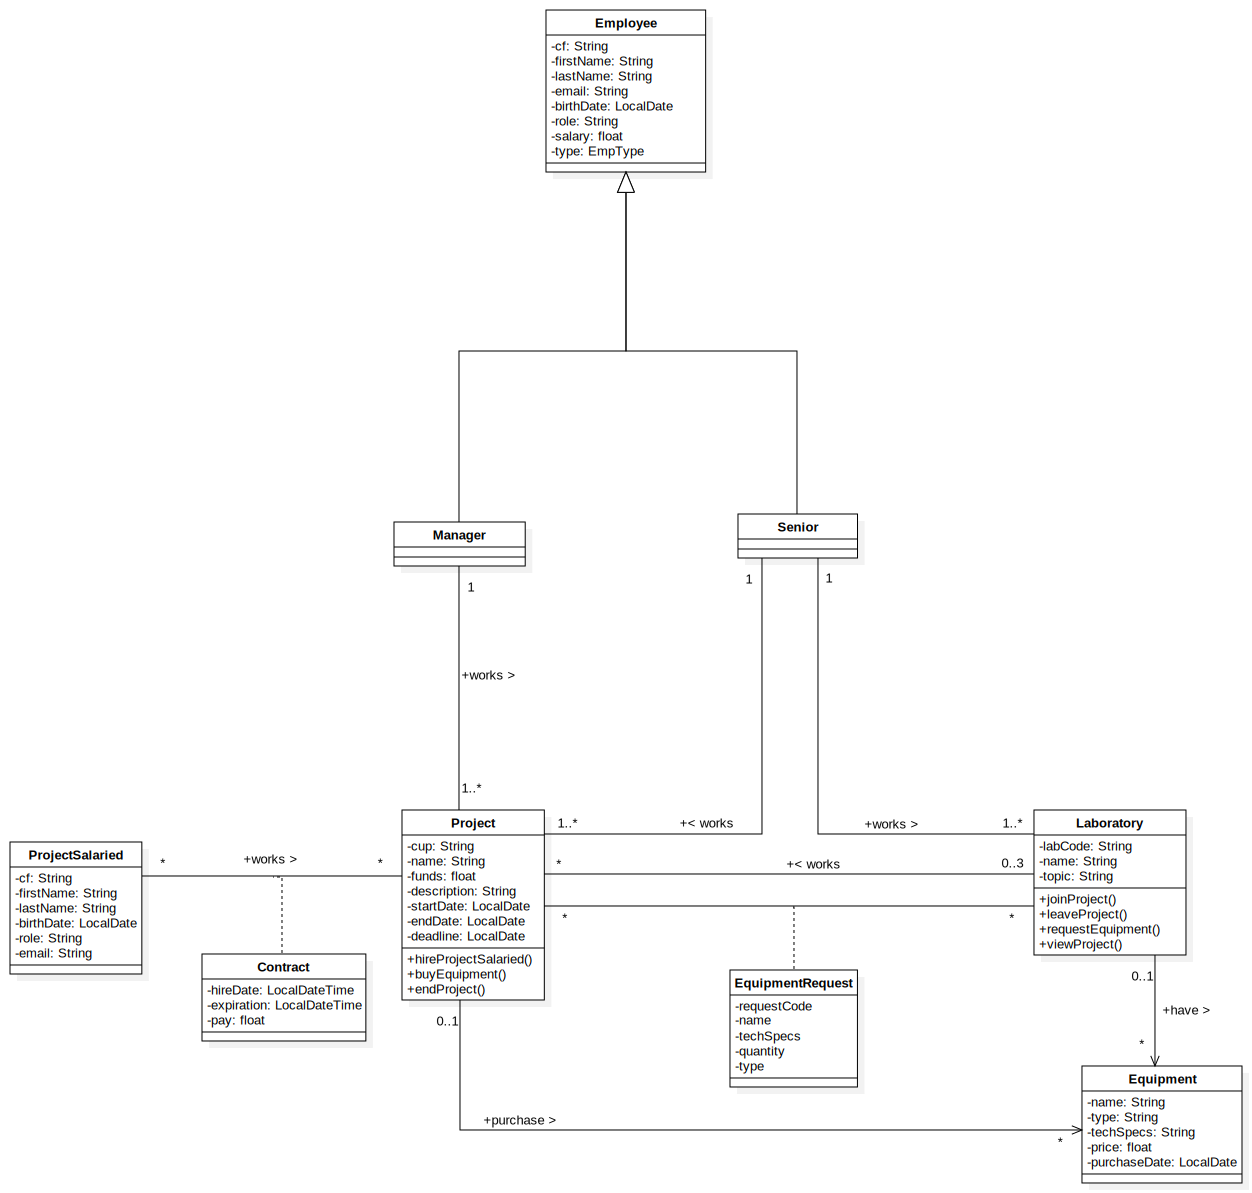
\includegraphics[width=\textwidth]{images/dominio_soluzione.png}

\section{Package diagram}
\includegraphics[width=\textwidth]{images/package_diagram.png}

\newpage
\section{Sequence diagrams}
\subsection{Leave Project}
Partendo dalla schermata di un utente senior, si seleziona un laboratorio e di quel laboratorio si seleziona il progetto che si desidera abbandonare.\\
Appare un alert dove l'utente decide di lasciare il progetto.\medskip \\
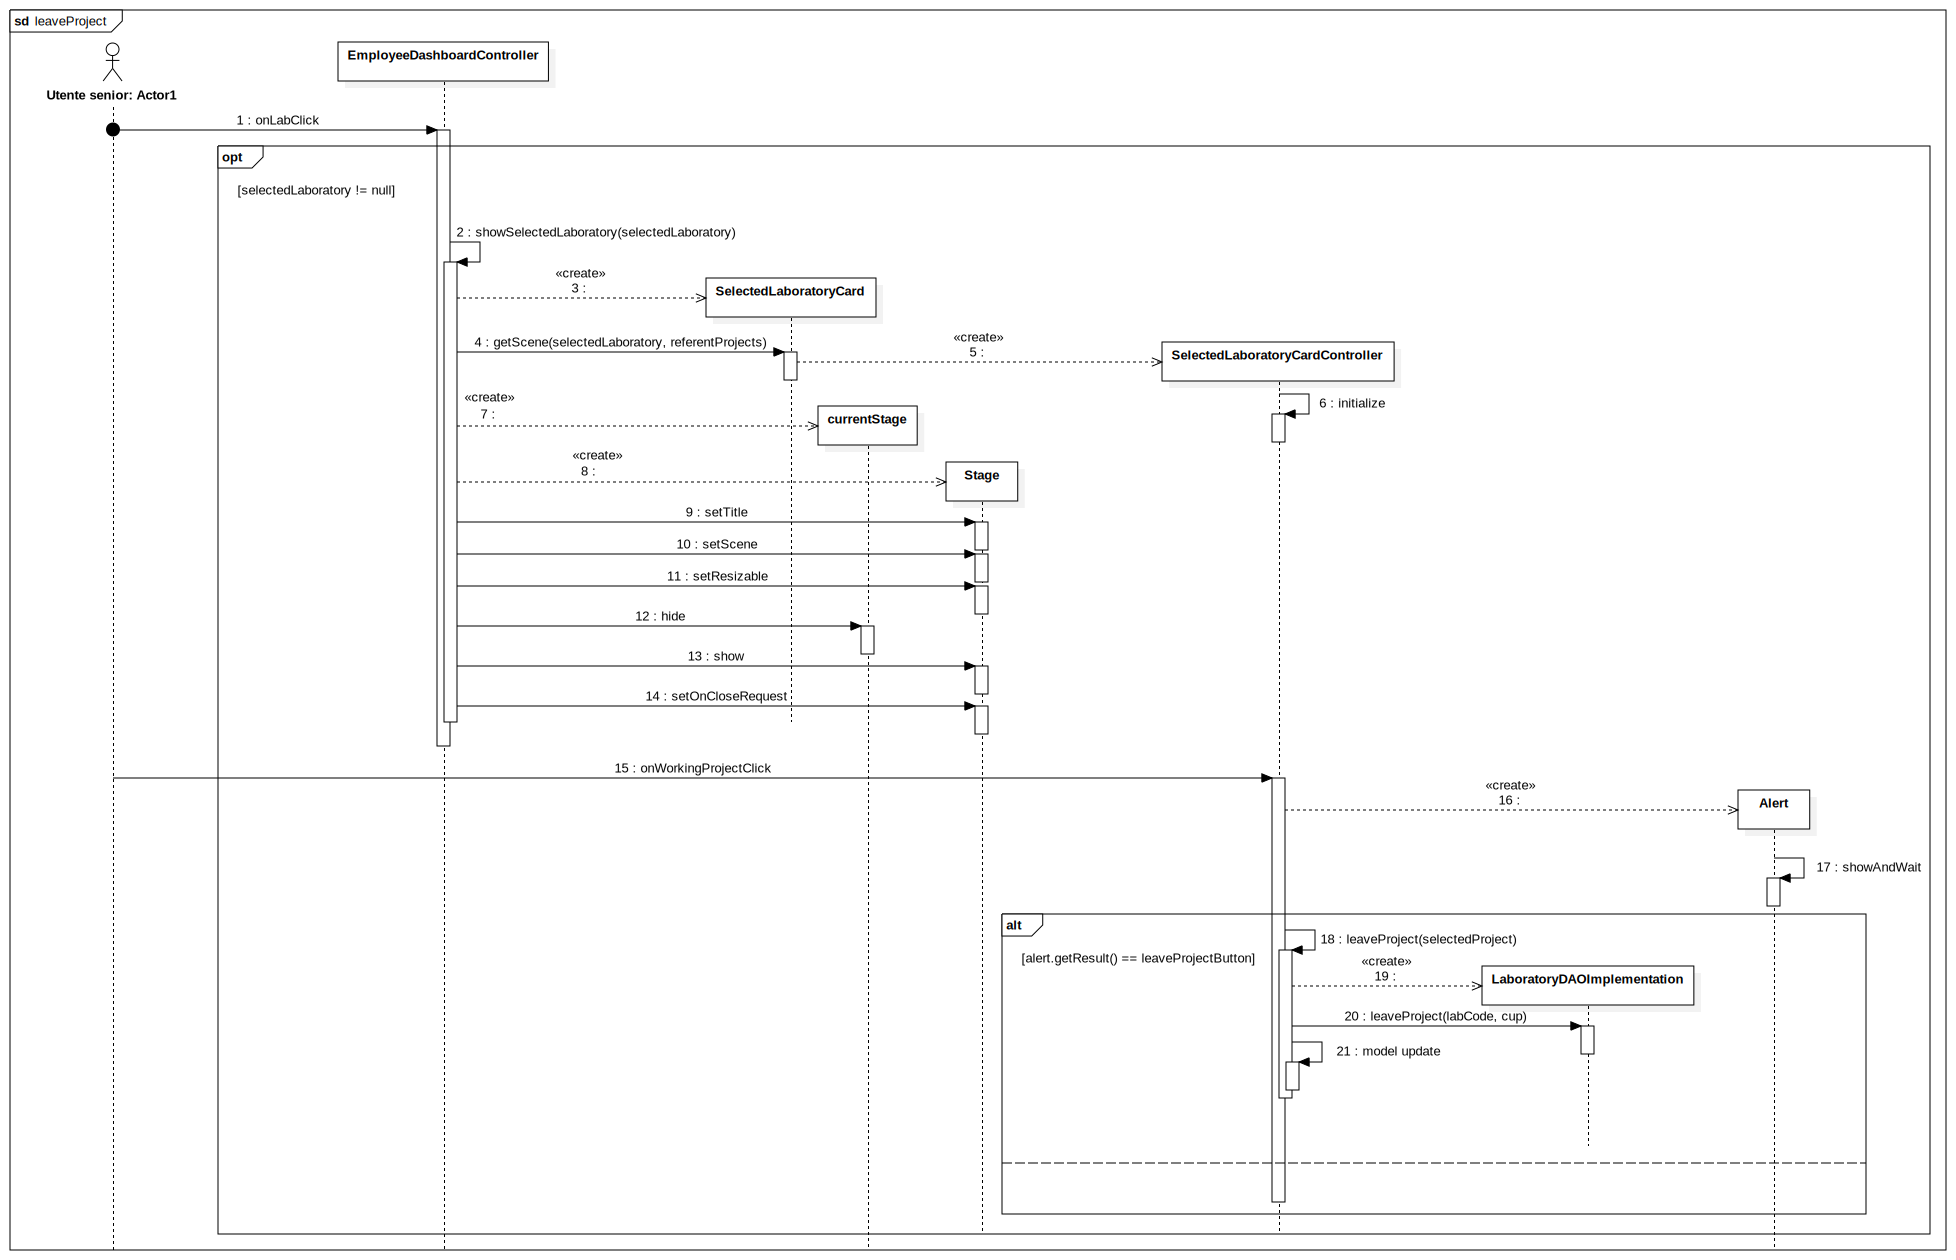
\includegraphics[width=\textwidth]{images/sequence_diagram_1.png}\newpage

\subsection{Employee Hiring}
Partendo dalla schermata di un utente senior oppure manager, si seleziona il pulsante di assunzione e si compilano i campi dell'impiegato che si vuole assumere. \\
In alternativa si può assumere un impiegato selezionado l'impiegato già assunto in precedenza dalla tabella, assumendolo nuovamente con un nuovo contratto.
\medskip \\
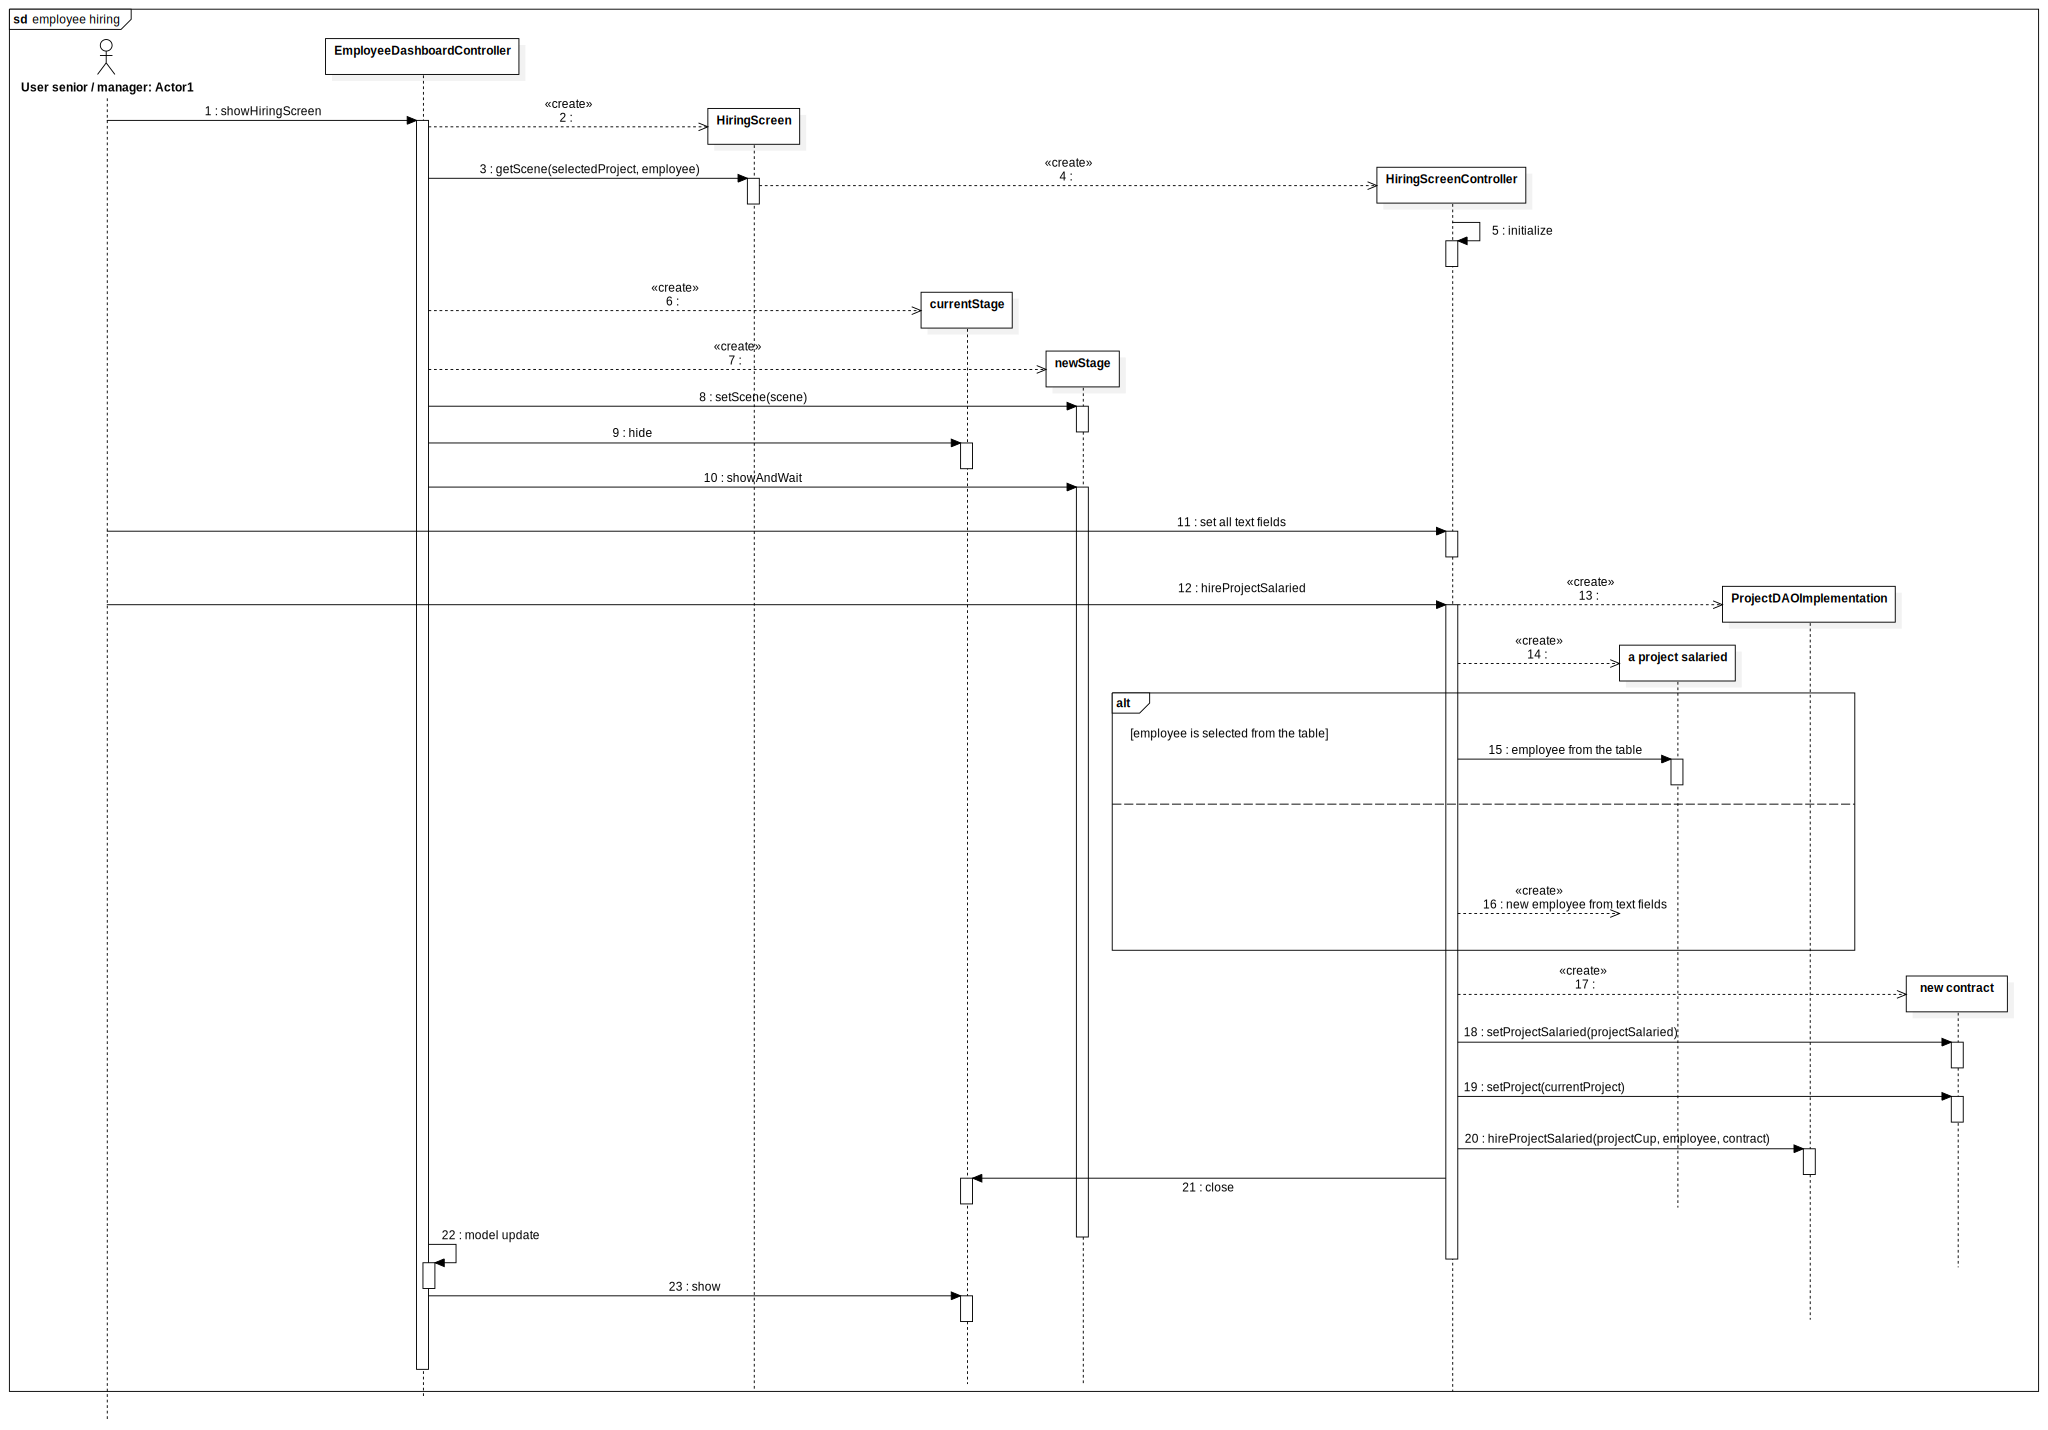
\includegraphics[width=\textwidth]{images/sequence_diagram_2.png}

\end{document}